% Chapter Template

\chapter{存储分离} % Main chapter title

\label{Chapter3} % Change X to a consecutive number; for referencing this chapter elsewhere, use \ref{ChapterX}

%----------------------------------------------------------------------------------------
%	SECTION 1
%----------------------------------------------------------------------------------------
\section{资源存储的背景与发展}
资源存储策略近年来不断发展更新,其发展路线符合资源分离的理念。
%-----------------------------------
%	SUBSECTION 1
%-----------------------------------
\subsection{直连式存储}

直连式存储(Direct-attached storage, DAS)是将外置存储设备通过小型计算机系统接口(Small computer system interface, SCSI)
直接连接到服务器主机上的资源存储方式,其特征是服务器主机与存储资源一体化。
由于服务器主机与存储设备是通过物理连接,主机访问硬盘资源的速度很快。
物理连接也是最为简单直接的连接方式,实现便捷,不需要专业人员的维护,能节省维护成本。
但服务器主机的SCSI ID资源很有限,能够与之通过DAS方式连接的存储设备是有限的,所以每台服务器主机所能管理的存储资源有上限,存储资源扩展性很差。
随着业务的不断发展,当数据量达到一定规模后,一台主机的存储资源便不足以满足业务需求,此时SCSI接口数量的限制成为瓶颈。
如果采用多台服务器来分布式存储数据,由于存储空间不能跨服务器动态分配,容易造成服务器负载不均衡和资源的浪费,且难于维护。
此外,由于服务器主机与存储设备一对多的关系,使得服务器主机一旦发生故障,所有数据都将不可访问,造成较大的影响。
(图~\ref{fig:das_architecture})为DAS架构图。

\begin{figure}
\centering
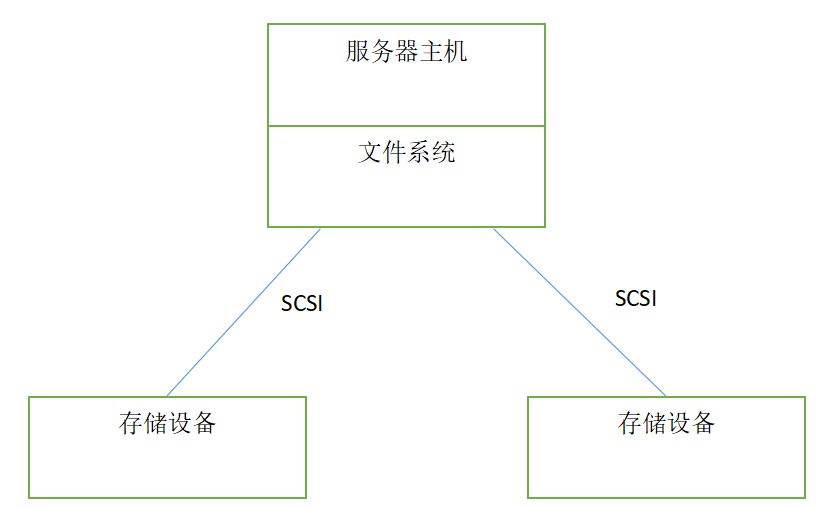
\includegraphics[scale=0.45]{Figures/storage/das_architecture.jpg}
\decoRule
\caption{DAS架构}
\label{fig:das_architecture}
\end{figure}

%-----------------------------------
%	SUBSECTION 2
%-----------------------------------
\subsection{存储区域网络}

存储区域网络(Storage Area Network, SAN)是通过网状通道(Fibre Channel, FC)交换机连接外置存储设备,建立专用于数据存储的区域网络。
在SAN模式下,服务器主机通过TCP/IP协议与存储设备通信。相比于DAS模式,SAN模式的基础是一个专用网络,可以自由地在SAN系统中添加存储设备,可扩展性大大加强。
(图~\ref{fig:san_architecture})为SAN架构图。

\begin{figure}
\centering
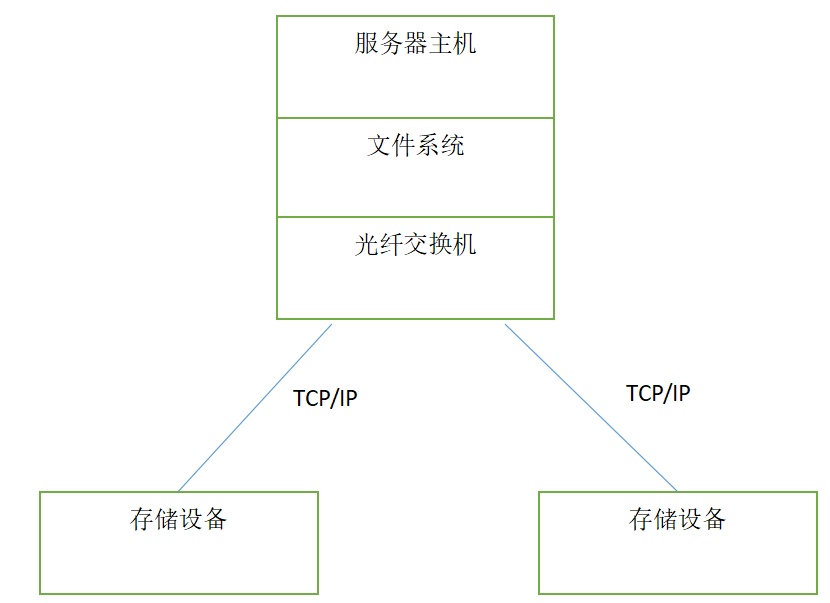
\includegraphics[scale=0.45]{Figures/storage/san_architecture.jpg}
\decoRule
\caption{SAN架构}
\label{fig:san_architecture}
\end{figure}

%-----------------------------------
%	SUBSECTION 3
%-----------------------------------
\subsection{网络附属存储}

网络附属存储(Network Attached Storage, NAS)是采用网络技术(TCP/IP, ATM, FDDI等)通过网络交换机连接存储系统和服务器主机来建立存储私网的存储模式。
NAS模式与SAN模式最大的区别在于NAS模式的文件系统位于存储设备端,其网络带宽消耗较大。
(图~\ref{fig:nas_architecture})为NAS架构图。

\begin{figure}
\centering
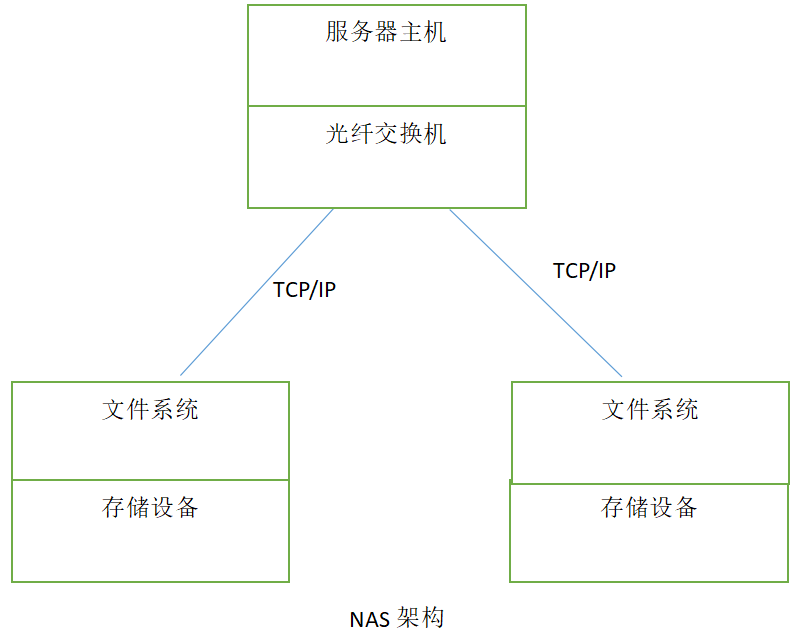
\includegraphics[scale=0.45]{Figures/storage/nas_architecture.jpg}
\decoRule
\caption{NAS架构}
\label{fig:nas_architecture}
\end{figure}

%-----------------------------------
%	SUBSECTION 4
%-----------------------------------
\subsection{发展分析}
纵观存储资源模式的发展历程,从DAS的各资源一体化,到SAN的存储资源网络化,再到NAS的文件系统网络化,存储资源的解耦程度越来越高。
这与存储资源分离(Storage Resource Disaggregation)的理念不谋而合。
存储资源分离使得存储设备从一体化的硬件中独立出去,通过控制器(Controller)转发网络信息实现与服务器主机的通信。
这样的设计能让控制器按照不同的策略动态分配存储资源的使用(如均衡化负载或集中化负载),有效缓解存储资源利用率低和存储资源不足等问题。
存储资源分离这一话题久盛不衰,许多学者在该领域从事研究工作,我们将以Klimovic等人\cite{klimovic2016flash}的工作为切入点,浅谈存储资源分离的发展和现状。

%----------------------------------------------------------------------------------------
%	SECTION 2
%----------------------------------------------------------------------------------------

\section{闪存资源分离(Flash Storage Disaggregation)}

%-----------------------------------
%	SUBSECTION 1
%-----------------------------------
\subsection{架构设计}

图~\ref{fig:d-a_flash_architecture}展示了传统的每台主机拥有一块闪存设备的架构,这意味着应用只能访问到对应的直连的闪存设备。
图~\ref{fig:dis_flash_architecture}是分离式闪存架构,其特点是闪存层(Flash Tier)从数据存储层(DataStore Tier)中解耦出来,
使得主机能够通过网络小型计算机接口(internet small computer system interface)访问所有的闪存设备,
并在闪存层增加协调管理器(coordination manager),负责选择合理的存储资源,以达到提高闪存资源利用率的目的。

\begin{figure}
\centering
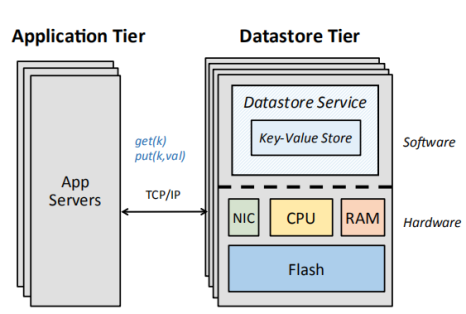
\includegraphics[scale=0.8]{Figures/storage/d-a_flash_architecture.jpg}
\decoRule
\caption{直连式闪存架构}
\label{fig:d-a_flash_architecture}
\end{figure}

\begin{figure}
\centering
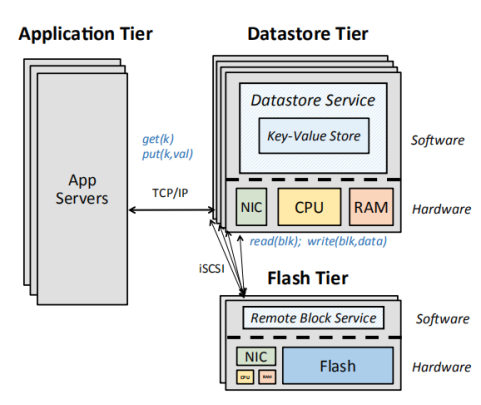
\includegraphics[scale=0.8]{Figures/storage/dis_flash_architecture.jpg}
\decoRule
\caption{分离式闪存架构}
\label{fig:dis_flash_architecture}
\end{figure}

%-----------------------------------
%	SUBSECTION 2
%-----------------------------------
\subsection{读写流程}
%-----------------------------------
%	SUBSUBSECTION 1
%-----------------------------------
\subsubsection{写流程}
iSCSI层的initiator能控制传输数据的时间,数据存储层维护一个指向协议数据单元(Protocol Data Unit, PDU)的指针。
iSCSI层对要写的数据进行包装(加入信息头等),然后由内核将PDU传输给闪存层。
其中包括的NIC和SCSI的缓存读写则取决与TCP/IP栈的实现。
%-----------------------------------
%	SUBSUBSECTION 2
%-----------------------------------
\subsubsection{读流程}
iSCSI的initiator接收到来自闪存层的包后,将使用DMA(Direct Memory Access)技术将包的数据从NIC模块转移至内核内存。
内核解析获取的包,拆离出数据内容,将之放在iSCSI的PDU。iSCSI层将PDU数据复制到SCSI缓存。
此时应用就可以从SCSI缓存中直接获取数据。

%-----------------------------------
%	SUBSECTION 3
%-----------------------------------
\subsection{性能评估}
%-----------------------------------
%	SUBSUBSECTION 1
%-----------------------------------
\subsubsection{延迟分析}
数据存储层使用RocksDB键值存储,利用mutilate负载生成器\cite{leverich2014mutilate}生成大量用户进程,进行大量的查询操作,
营造期望的每秒查询率(Queries Per Second, QPS)。图~\ref{fig:read_latency_CDF}展示了在无负载系统下,
本地闪存与远程闪存读取数据的用户延迟的累积分布函数(Cumulative Distribution Function)。
远程闪存的用户延迟显然高于本地闪存,在曲线的95\%处,远程闪存读取延迟约比本地闪存高260微秒。
由于延迟SLA在5到10毫秒左右,远远高于微秒数量级,所以远程闪存的延迟代价在可接受范围内。

\begin{figure}
\centering
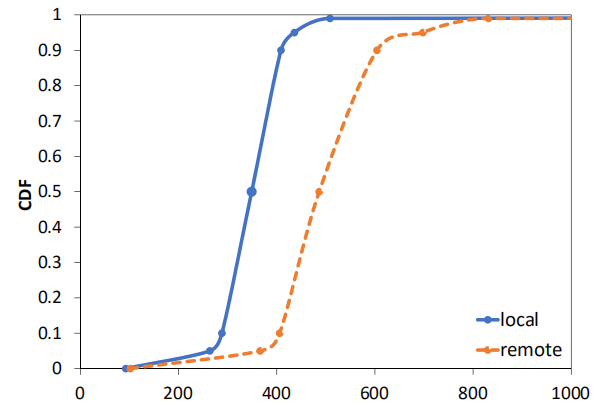
\includegraphics[scale=0.8]{Figures/storage/read_latency_CDF.jpg}
\decoRule
\caption{读操作延迟的CDF曲线}
\label{fig:read_latency_CDF}
\end{figure}

%-----------------------------------
%	SUBSUBSECTION 2
%-----------------------------------
\subsubsection{吞吐量分析}
为测试本地闪存和远程闪存的吞吐量指标,控制应用层的每秒请求率(QPS),并描绘点(QPS,延迟),图~\ref{fig:QPS_latency}展示其吞吐量性能。
由图分析,在相同延迟情况下,远程闪存吞吐量约为本地闪存的80\%。表观上,远程闪存的吞吐量受到了较严重的影响。
一方面,这是存储设备性能和资源利用率等的权衡,远程闪存的理念是牺牲了部分性能,换取更好的资源利用率。
另一方面,可以通过扩展数据存储层的CPU来补偿这些吞吐量损失。

\begin{figure}
\centering
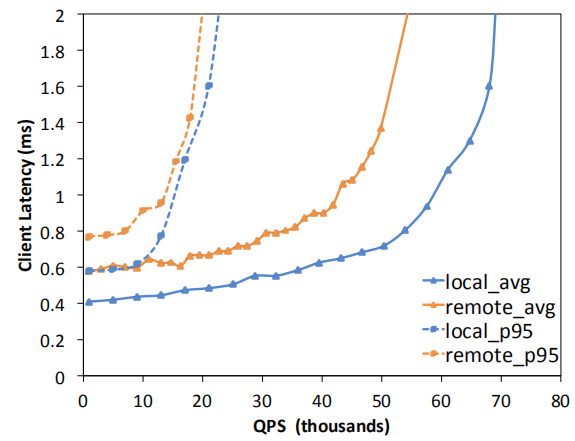
\includegraphics[scale=0.8]{Figures/storage/QPS_latency.jpg}
\decoRule
\caption{单SSDB服务器的延迟-QPS曲线}
\label{fig:QPS_latency}
\end{figure}

%-----------------------------------
%	SUBSUBSECTION 3
%-----------------------------------
\subsubsection{敏感度分析}
通过在SSDB中增加循环进程,创造不同CPU负载的环境,测试远程闪存的QPS对不同参数的曲线变化率(敏感度)。
图~\ref{fig:QPS_CPUintensity}展示了本地闪存和远程闪存在不同CPU负载下的QPS。二者在CPU负载较低的环境下,本地闪存较远程闪存有更高的QPS,
意味着远程闪存的性能受到一定影响,而在CPU处于较高负载的环境下,本地闪存与远程闪存的QPS相差无几,
意味着此时主要瓶颈不在iSCSI通讯上。同时,本地闪存的QPS受CPU负载大小的影响比远程闪存大,也就是说,远程闪存的性能表现更加稳定。


图~\ref{fig:QPS_percentage}展示了在相同请求数量下,本地闪存和远程闪存的QPS随写请求占总请求的比例变化曲线。
二者的QPS都随着写请求比例增加而增加,因为写操作的返回是异步的,其效率比读操作高。
二者的QPS差值在不同的写操作比例下差别不大,可以得出结论,读写操作所占比例对本地闪存和远程闪存性能差距影响不大。

\begin{figure}
\centering
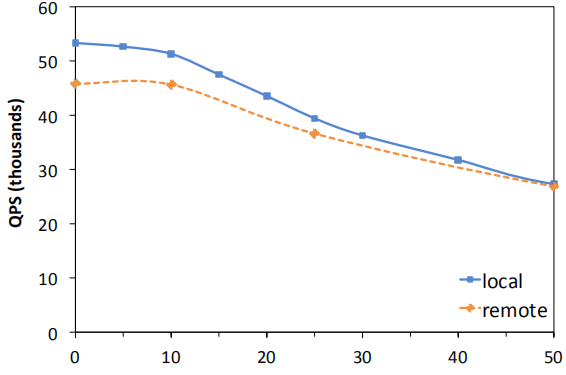
\includegraphics[scale=0.8]{Figures/storage/QPS_CPUintensity.jpg}
\decoRule
\caption{QPS随CPU负载变化曲线}
\label{fig:QPS_CPUintensity}
\end{figure}

\begin{figure}
\centering
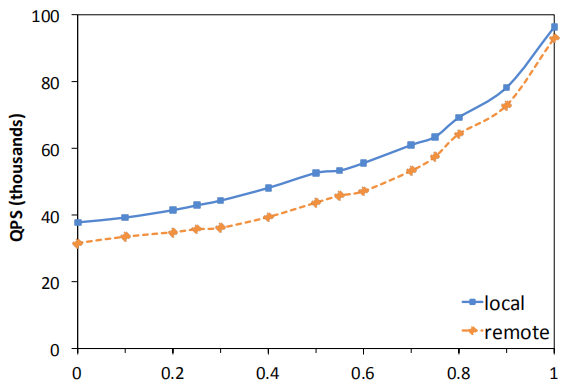
\includegraphics[scale=0.8]{Figures/storage/QPS_percentage.jpg}
\decoRule
\caption{QPS随读操作占比变化曲线}
\label{fig:QPS_percentage}
\end{figure}

%-----------------------------------
%	SUBSUBSECTION 4
%-----------------------------------
\subsubsection{多服务端性能分析}
实际情况中,机群中服务器主机与闪存时多对多的关系,所以分析多服务端共享同闪存集群的性能很有实际价值。
图~\ref{fig:2SSDB_latency_QPS}和图~\ref{fig:3SSDB_latency_QPS}分别展示两个SSDB服务器主机和三个SSDB服务器主机时,本地闪存与远程闪存的延迟-QPS曲线图。
毫无疑问,本地闪存的QPS性能始终比远程闪存更高。值得一提的是,三个SSDB环境相较于两个SSDB环境下,远程闪存的QPS性能损失代价更严重。

\begin{figure}
\centering
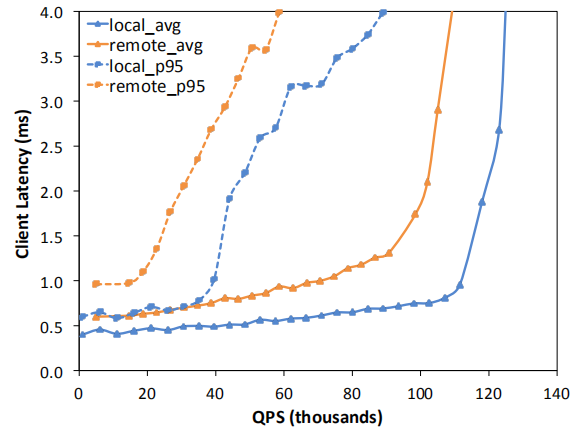
\includegraphics[scale=0.8]{Figures/storage/2SSDB_latency_QPS.jpg}
\decoRule
\caption{2个SSDB服务共享闪存下,延迟-QPS曲线}
\label{fig:2SSDB_latency_QPS}
\end{figure}

\begin{figure}
\centering
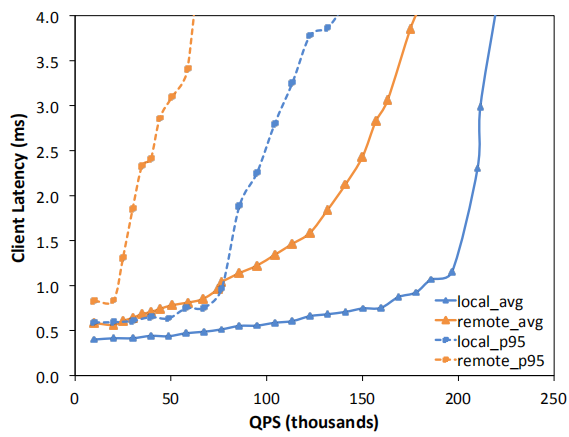
\includegraphics[scale=0.8]{Figures/storage/3SSDB_latency_QPS.jpg}
\decoRule
\caption{3个SSDB服务共享闪存下,延迟-QPS曲线}
\label{fig:3SSDB_latency_QPS}
\end{figure}

%-----------------------------------
%	SUBSECTION 4
%-----------------------------------
\subsection{存储分离适用情境分析}
通过计算直连式闪存(Direct-attached flash)和远程闪存(disaggregation flash)的主要消耗C$_{direct}$和C$_{disagg}$,对存储分离进行优势评估。
直连式闪存的消耗包括闪存读写的消耗和数据存储端CPU、RAM、NIC的消耗两部分,远程闪存则包括闪存读写的消耗,数据存储层CPU、RAM、NIC的消耗和闪存层CPU、RAM、NIC的消耗。
这些消耗的权重为目标数据与实际数据的比值,如目标QPS与实际QPS的比值。
计算而得的消耗越大,意味着其资源利用越差,反之则越好。
引入新的评估指标,消耗节约比例。
消耗节约比例含义为使用远程闪存比直连式闪存节约的消耗比例。
若消耗节约比例值为正,则表示该环境参数下远程闪存消耗比直连式闪存小;反之则远程闪存消耗更大。


图~\ref{fig:compute_storage}展示了在计算强度比例因子和存储空间比例因子分布空间下,相应的消耗节约比例。
由图例的对称性可以分析而得,闪存读写的消耗与数据存储层的CPU、RAM、NIC消耗大致相等。
在不同的情景假设下(对应图中不同的二维坐标),对资源的分配权衡也是不一样的。
若闪存资源的价值比CPU、内存低,那么服务器将倾向高闪存空间和低计算强度,对应图例的右下半边区域,该区域的消耗节约比例大于零,
意味着远程闪存消耗比直连式闪存低,则此情境下,服务器主机更适合于远程闪存。
若闪存资源的价值比CPU、内存高,那么服务器将倾向低闪存空间和高计算强度,对应图例的坐上半边区域,同理,该区域的消耗节约比例大于零,
远程闪存消耗比直连式闪存低,服务器主机更适合于远程闪存。
若闪存资源与CPU、内存资源价值相当,对应图例的对角线区域,该区域的消耗节约比例小于零,
也就是远程闪存消耗比直连式闪存高,此时服务器主机更适合直连式闪存。

\begin{figure}
\centering
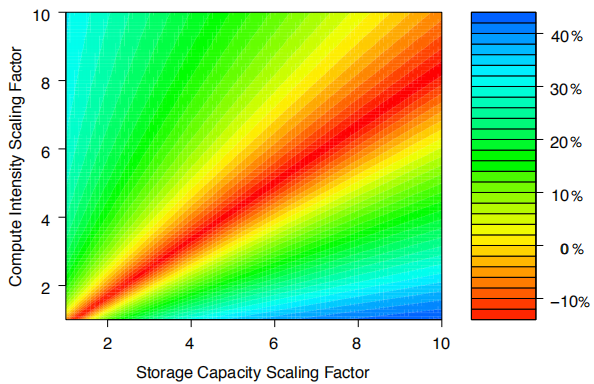
\includegraphics[scale=0.7]{Figures/storage/compute_storage.jpg}
\decoRule
\caption{消耗节约比例-计算强度比例因子-存储空间比例因子分布图}
\label{fig:compute_storage}
\end{figure}

%----------------------------------------------------------------------------------------
%	SECTION 2
%----------------------------------------------------------------------------------------

\section{本章小结}

Klimovic等人\cite{klimovic2016flash}对闪存分离策略做了充分的研究,分析了闪存分离带来的容量和资源利用率优势,也客观展示了资源分离带来的性能损失,
并提出了弥补性能损失的方法。事实上,在考虑服务器主机整体架构时,不能盲目地强调闪存分离的优势,忽略其带来的性能损失和维护成本。
分离式闪存与直连式闪存各有优劣。
更加客观的策略是,通过各类资源(如CPU,内存,闪存)的当前价值来定量计算分离式闪存带来的提升及损失孰重孰轻,进而合理取舍。















